%--------------------------------------------------------------------------------------------------
%
\chapter{Cross-lingual Document Similarity}\label{chap:crosslingual}
%--------------------------------------------------------------------------------------------------

Document similarity is an important component in techniques from text mining and natural language processing. Many techniques use the similarity as a black box, e.g., a kernel in Support Vector Machines. Comparison of documents (or other types of text snippets) in a monolingual setting is a well-studied problem in the field of information retrieval ~\cite{Salton88term-weightingapproaches}. We first formally introduce the problem followed by a description of  our approach.

\section{Problem definition}\label{sec:tfidf}
We will first describe how documents are represented as vectors and how to compare documents in a mono-lingual setting. We then define a way to measure cross-lingual similarity which is natural for the models we consider.

\noindent\textbf{Document representation.}
The standard vector space model~\cite{Salton88term-weightingapproaches} represents documents as vectors, where each term corresponds to a word or a phrase in a fixed vocabulary. Formally, document $d$ is represented by a vector $x \in \RR^n$, where $n$ corresponds to the size of the vocabulary, and vector elements $x_k$ correspond to the number of times term $k$ occurred in the document, also called \emph{term frequency} or $TF_k(d)$.

We also used a term re-weighting scheme that adjusts for the fact that some words occur more frequently in general. A term weight should correspond to the importance of the term for the given corpus. The common weighting scheme is called \emph{Term Frequency Inverse Document Frequency} ($TFIDF$) weighting. An \emph{Inverse Document Frequency} ($IDF$) weight for the dictionary term $k$ is defined as $\log\left( \frac{N}{DF_k} \right)$, where $DF_k$ is the number of documents in the corpus which contain term $k$.
When building cross-lingual models, the IDF scores were computed with respect to the Wikipedia corpus. In the other part of our system, we computed TFIDF vectors on streams of news articles in multiple languages. There the IDF scores for each language changed dynamically - for each new document we computed the IDF of all news articles within a 10 day window.

Therefore we can define a document's $TFIDF$ as
$$ x_{ij}  := \frac{\mbox{term frequency in document } i}{\mbox{inverse document frequency of term } j}.$$
The $TFIDF$ weighted vector space model document representation corresponds to a map $\phi : \text{text} \rightarrow \RR^n$ defined by:
$$\phi(d)_k = {TF}_k(d) \log\left( \frac{N}{{DF}_k}\right).$$

\noindent\textbf {Mono-lingual similarity.}
A common way of computing similarity between documents is \emph{cosine similarity},
$$sim(d_1, d_2) = \frac{\langle \phi(d_1), \phi(d_2)\rangle}{\|\phi(d_1)\| \|\phi(d_2)\|},$$
where $\langle \cdot,\cdot \rangle$ and $\|\cdot\|$ are standard inner product and Euclidean norm. When dealing with two or more languages, one could ignore the language information
and build a vector space using the union of tokens over the languages. A cosine similarity function in such a space can be useful to some extent, for example ``Internet'' or ``Obama'' may appear both in Spanish and English texts and the presence of such terms in both an English and a Spanish document would contribute to their similarity. In general however, large parts of vocabularies may not intersect. This means that given a language pair, many words in both languages cannot contribute to the similarity score. Such cases can make the similarity function very insensitive to the data.

\noindent\textbf {Cross-lingual similarity.}
Processing a multilingual dataset results in several vector spaces with varying dimensionality, one for each language. The dimensionality of the vector space corresponding to the $i$-th language is denoted by $n_i$ and the vector space model mapping is denoted by $\phi_i : \text{text} \rightarrow \RR^{n_i}$.
The similarity between documents in language $i$ and language $j$ is defined as a bilinear operator represented as a matrix $S_{i,j} \in \RR^{n_i \times n_j}$:
$$sim_{i,j}(d_1, d_2) = \frac{ \langle \phi_i (d_1), S_{i,j} \phi_j (d_2) \rangle }{\|\phi_i(d_1)\| \|\phi_j(d_2)\|},$$
where $d_1$ and $d_2$ are documents written in the $i$-th and $j$-th language respectively. If the maximal singular value of $S_{i,j}$ is bounded by $1$, then the similarity scores will lie on the interval $[-1, 1]$. We will provide an overview of the models in Section \ref{sec:models} and then introduce additional notation in \ref{sec:notation}. Starting with Section \ref{sec:kmeans} and ending with Section \ref{sec:hublang} we will describe some approaches to compute $S_{i,j}$ given training data.

\section{Cross-Lingual Models}\label{sec:models}
In this section, we will describe several approaches to the problem of computing the multilingual similarities introduced in Section~\ref{sec:tfidf}. We present four approaches:
a simple approach based on $k$-means clustering in Section~\ref{sec:kmeans}, a standard approach based on singular value decomposition in Section~\ref{sec:LSI}, a related
approach called Canonical Correlation Analysis (CCA) in Section~\ref{sec:CCA} and finally a new method, which is an extension of CCA to more than two languages in Section~\ref{sec:hublang}.
%
CCA can be used to find correlated patterns for a pair of languages, whereas the extended method optimizes a
Sum of Squared Correlations (SSCOR) between several language pairs, which was introduced in~\cite{Kettenring}. The SSCOR problem is difficult to solve in our setting (hundreds of thousands of features, hundreds of thousands of examples). To tackle this, we propose a method which consists of two ingredients.
 The first one is based on an observation that certain datasets (such as Wikipedia) are biased towards one language (English for Wikipedia), which can be exploited
 to reformulate a difficult optimization problem as an eigenvector problem. The second ingredient is dimensionality reduction using CL-LSI, which
 makes the eigenvector problem computationally and numerically tractable.

We concentrate on approaches that are based on linear maps rather than alternatives, such as machine translation and probabilistic models, as discussed in the section on related work.
We will start by introducing some notation.

\section{Notation}\label{sec:notation}

The cross-lingual similarity models presented in this paper are based on comparable corpora. A \emph{comparable corpus} is a collection of documents in multiple languages, with alignment between documents that are of the same topic, or even a rough translation of each other. Wikipedia is an example of a comparable corpus, where a specific entry can be described in multiple languages (e.g., ``Berlin" is currently described in 222 languages). News articles represent another example, where the same event can be described by newspapers in several languages.

More formally, a \emph{multilingual document} $d = (u_1,\ldots u_m)$ is a tuple of $m$ documents on the same topic (comparable), where $u_i$ is the document written in language $i$. Note that an individual document $u_i$ can be an empty document (missing resource) and each $d$ must contain at least \textbf{two nonempty documents}. This means that in our analysis we discard strictly monolingual documents for which no cross-lingual information is available. A comparable corpus $D = {d_1, \ldots, d_s}$ is a collection of $s$ multilingual documents. By using the vector space model, we can represent $D$ as a set of $m$ matrices $X_1,\ldots,X_m$, where $X_i \in \RR^{n_i \times s}$ is the matrix corresponding to the language $i$ and $n_i$ is the vocabulary size of language $i$. Furthermore, let $X_i^{\ell}$ denote the $\ell$-th column of matrix $X_i$ and the matrices respect the document alignment - the vector $X_i^\ell$ corresponds to the TFIDF vector of the $i$-th component of multilingual document $d_\ell$. We use $N$ to denote the total row dimension of $X$, i.e., $N:= \sum_{i=1}^m n_i$. See Figure~\ref{fig:stacked_matrices} for an illustration of the introduced notation.

\begin{figure}[tbp]
\centering
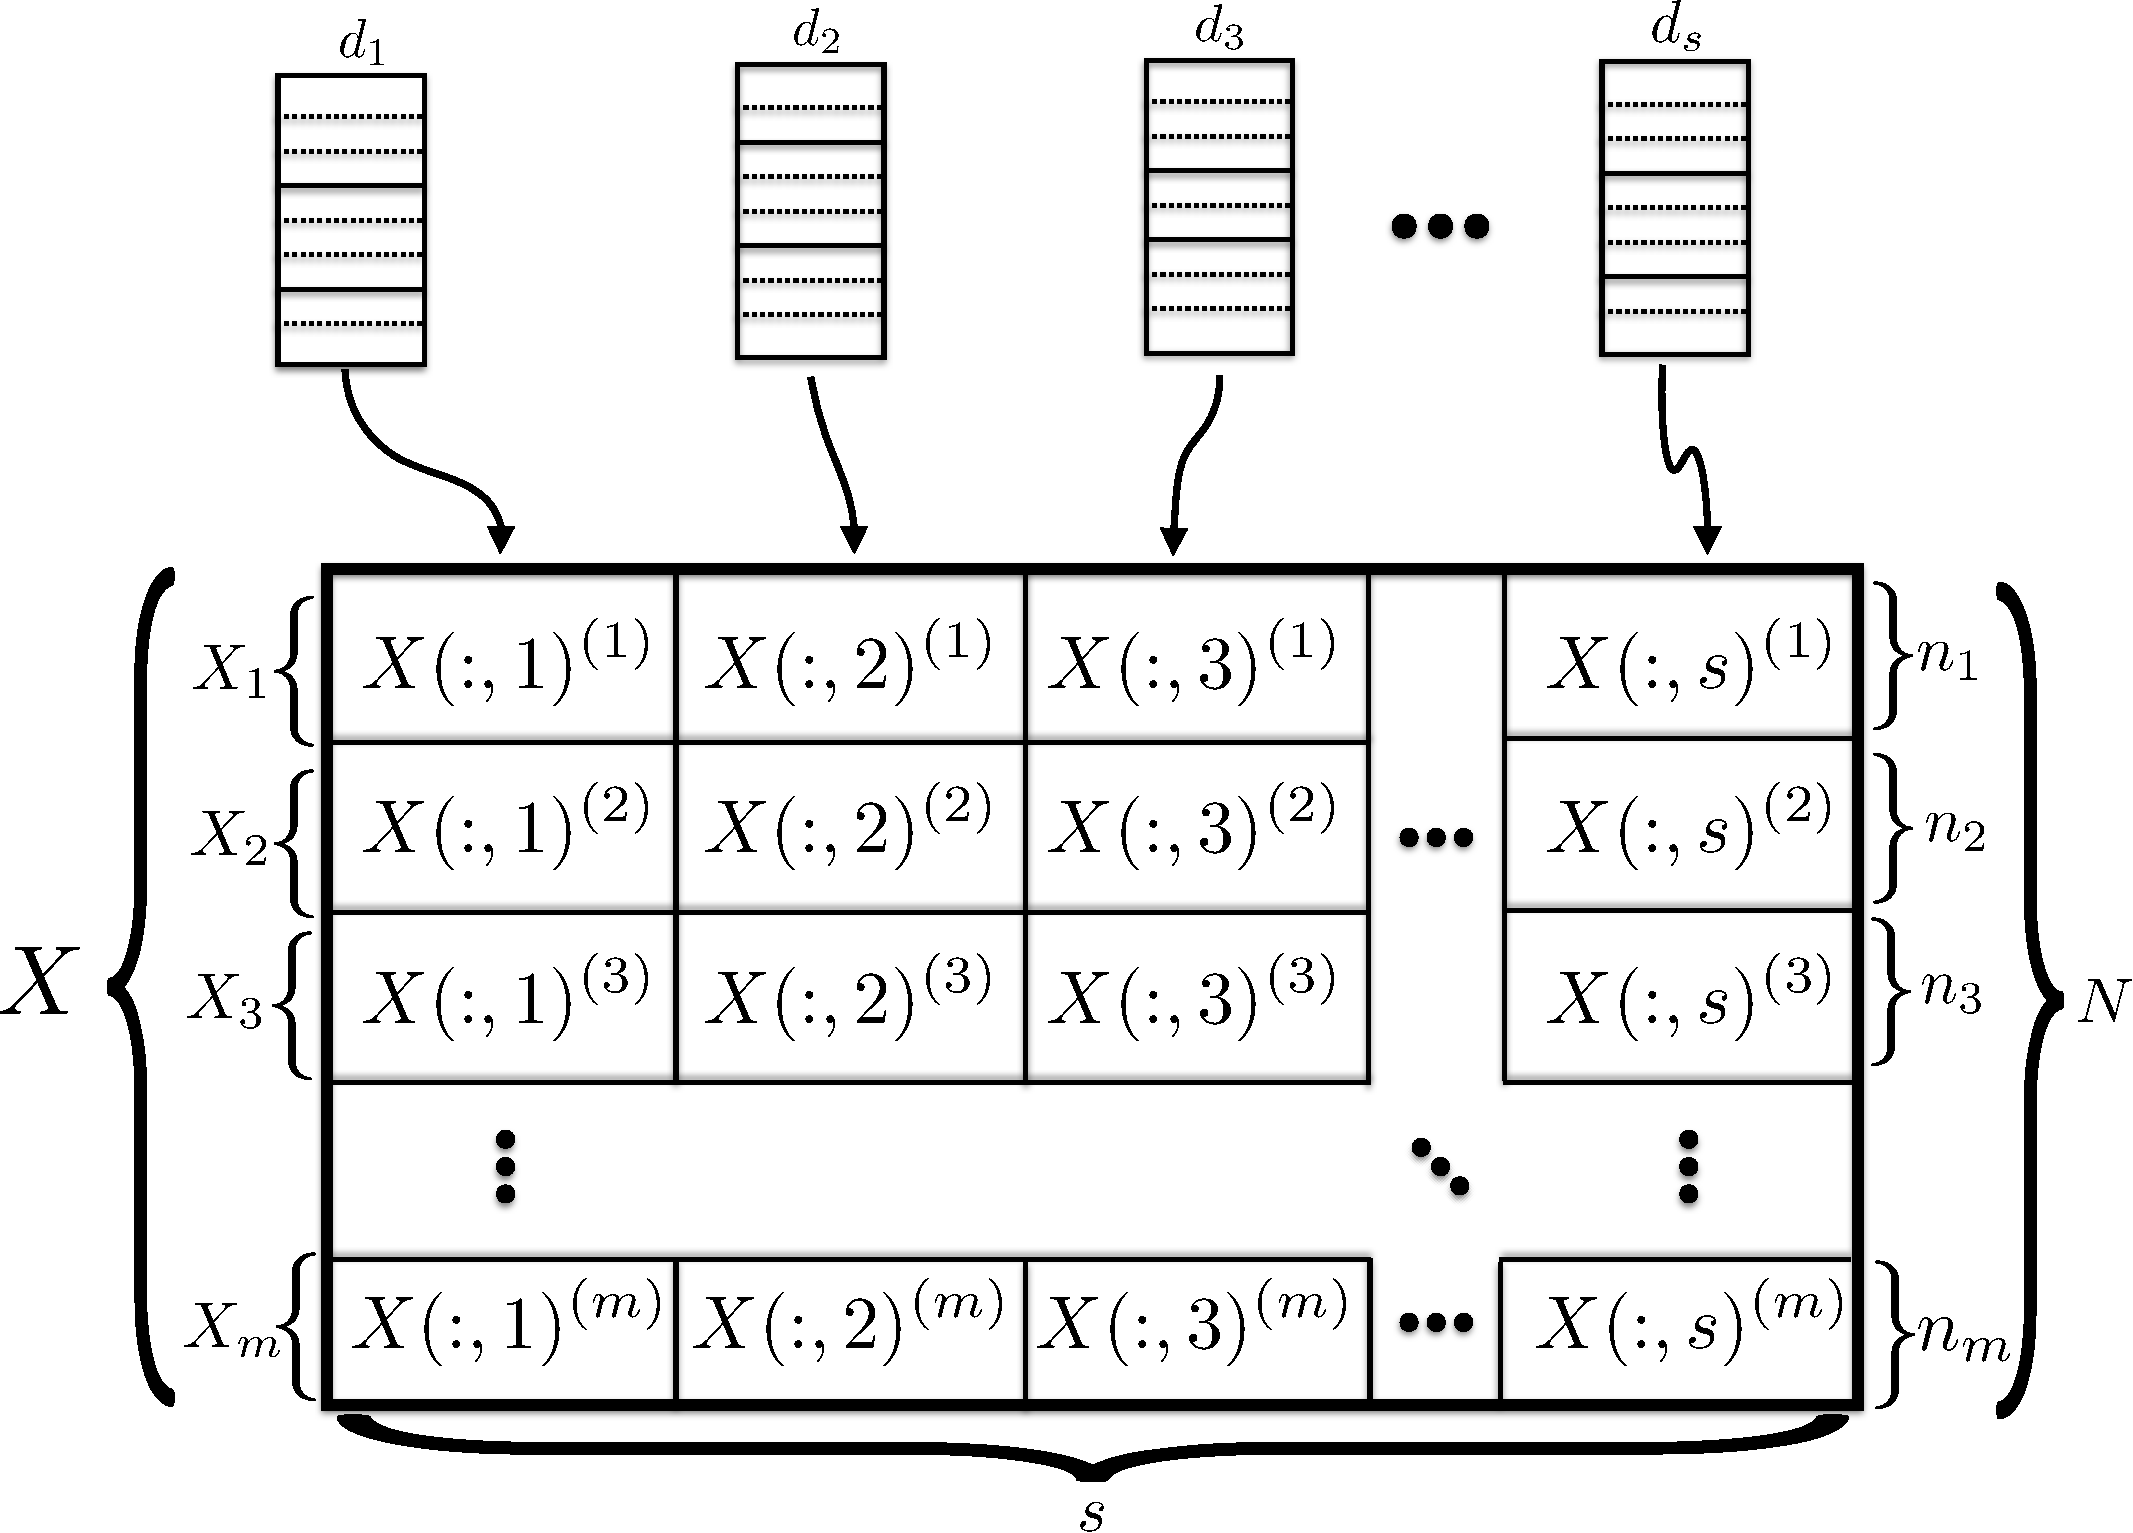
\includegraphics[width=9cm]{figures/stacked_matrices1-crop.pdf}
\caption{\label{fig:stacked_matrices} Multilingual corpora and their matrix representations using the vector space model.}
\end{figure}

We will now describe four models to cross-lingual similarity computation in the next sub-sections.
\section{$k$-means}\label{sec:kmeans}

The $k$-means algorithm is perhaps the most well-known and widely-used clustering algorithm. Here, we present its application
to compute cross-lingual similarities. The idea is based on concatenating the corpus matrices, running standard $k$-means clustering to obtain the matrix of centroids, ``reversing" the concatenation step to obtain a set of aligned bases, which are finally used to compute cross-lingual similarities. See Figure~\ref{fig:kmeans} for overview of the procedure. The left side of Figure~\ref{fig:kmeans} illustrates the decomposition and the right side summarizes the coordinate change.

\begin{figure}[tbp]
\centering
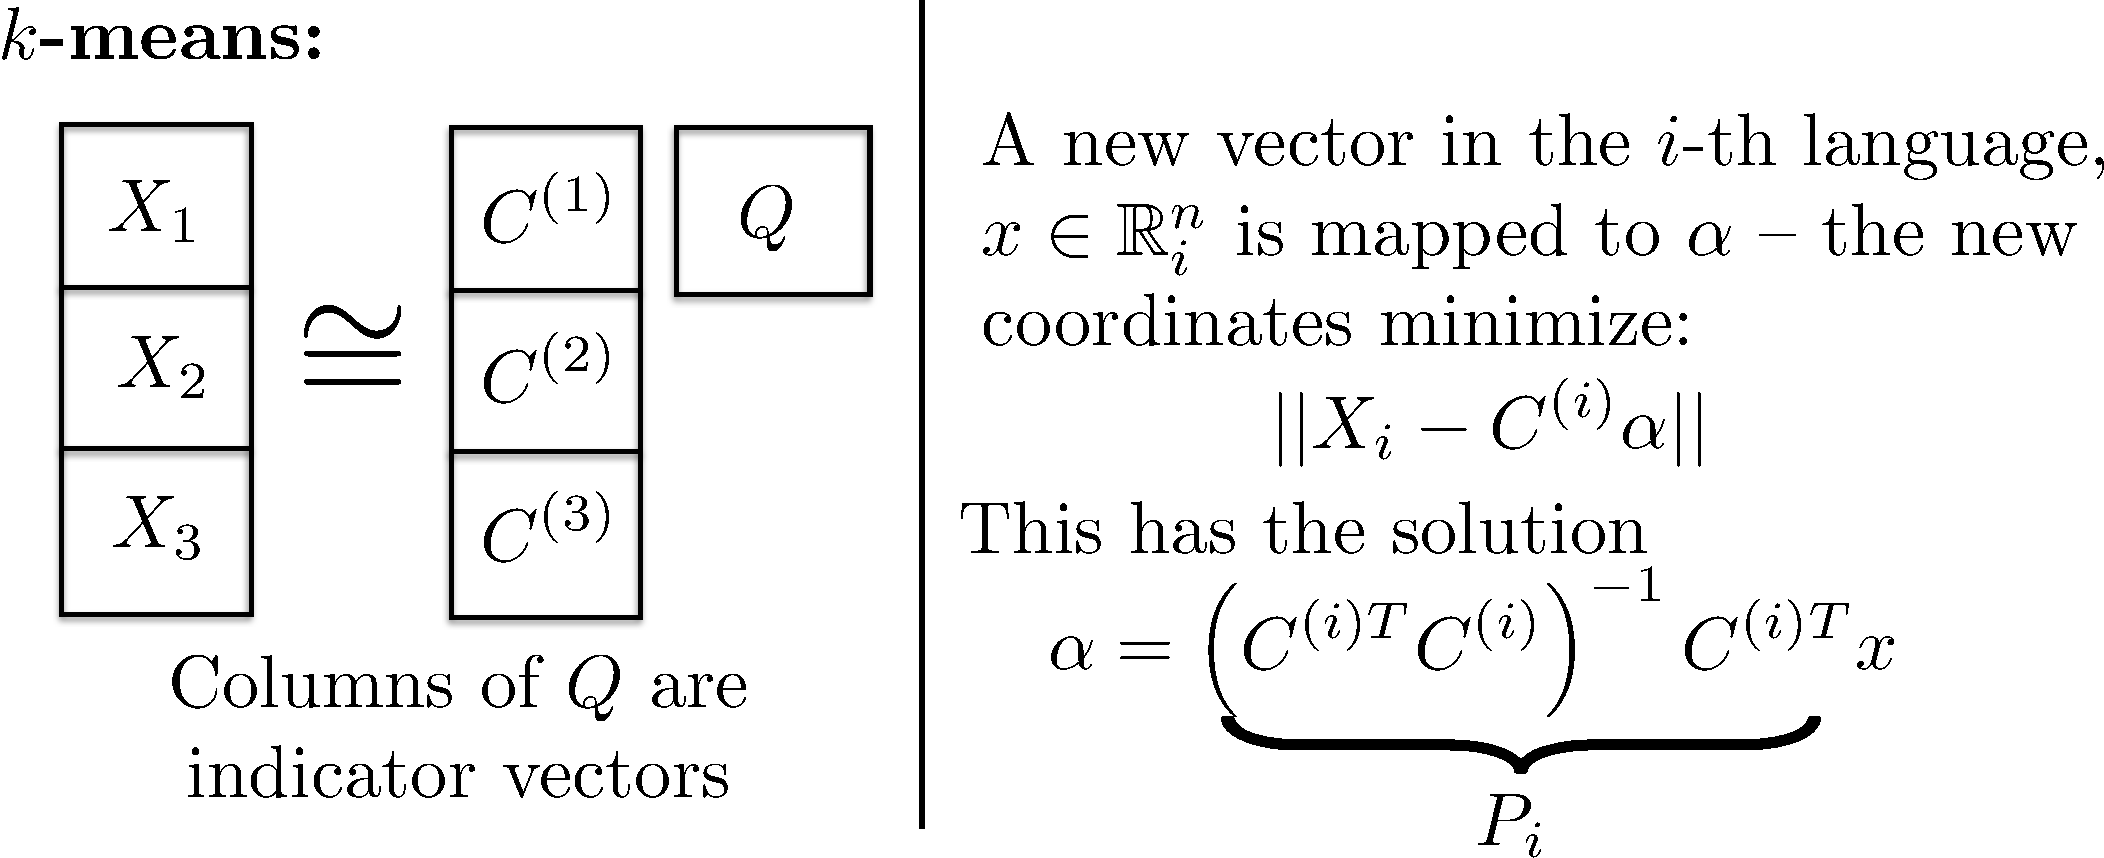
\includegraphics[width=10cm]{figures/kmeans.pdf}
\caption{\label{fig:kmeans} $k$-means algorithm and coordinate change.}
\end{figure}

 In order to apply the algorithm, we first merge all the term-document matrices into a single matrix $X$ by stacking the individual term-document matrices (as seen in Figure~\ref{fig:stacked_matrices}):
$$X := \begin{bmatrix}X_1^T ,X_2^T, \cdots, X_m^T \end{bmatrix}^T,$$
such that the columns respect the alignment of the documents (here MATLAB notation for concatenating matrices is used). Therefore, each document  is represented by a long vector indexed by the terms in all languages.

We then run the $k$-means algorithm~\cite{kmeans} and obtain a centroid matrix $C \in \RR^{N \times k}$, where the $k$ columns represent centroid vectors. The centroid matrix can be split vertically into $m$ blocks: $$C = [C_1^T \cdots C_m^T]^T,$$ according to the number of dimensions of each language, i.e., $C_i \in \RR^{n_i \times k}$.
%
To reiterate, the matrices $C_i$ are computed using a multilingual corpus matrix $X$ (based on Wikipedia for example).

To compute  cross-lingual document similarities on new documents, note that each matrix $C_i$ represents a vector space basis and can be used to map points in $\RR^{n_i}$ into a $k$-dimensional space, where the new coordinates of a vector $x \in \RR^{n_i}$ are expressed as: $$(C_i^T C_i)^{-1} C_i^T x_i.$$

The resulting matrix for similarity computation between language $i$ and language $j$ is defined up to a scaling factor as:
$$C_i(C_i^T C_i)^{-1} (C_j^T C_j)^{-1} C_j.$$

The matrix is a result of mapping documents in a language independent space using pseudo-inverses of the centroid matrices $P_i = (C_i^T C_i)^{-1} C_i$ and then comparing them using the standard inner product, which results in the matrix $P_i^T P_j$. For the sake of presentation, we assumed that the centroid vectors are linearly independent. (An independent subspace could be obtained using an additional Gram-Schmidt step~\cite{golub} on the matrix $C$, if this was not the case.)

\section{Cross-Lingual Latent Semantic Indexing}\label{sec:LSI}

The second approach we consider is Cross-Lingual Latent Semantic Indexing (CL-LSI)~\cite{cl_lsi} which is a variant of LSI~\cite{lsi} for more than one language. The approach is very similar to $k$-means, where we first concatenate the corpus matrices, compute a decomposition, which in case of CL-LSI is a truncated Singular Value Decomposition (SVD), decouple the
 column space matrix and use the blocks to compute linear maps to a common vector space, where standard cosine similarity is used to compare documents.

 The method is based on computing a truncated singular value decomposition of the concatenated corpus matrix $X \approx U S V^T$. See Figure~\ref{fig:lsi} for the decomposition. Representing documents in ``topic`` coordinates is done in the same way as in the $k$-means case (see Figure~\ref{fig:kmeans}), we will describe how to compute the coordinate change functions.

\begin{figure}[tbp]
\centering
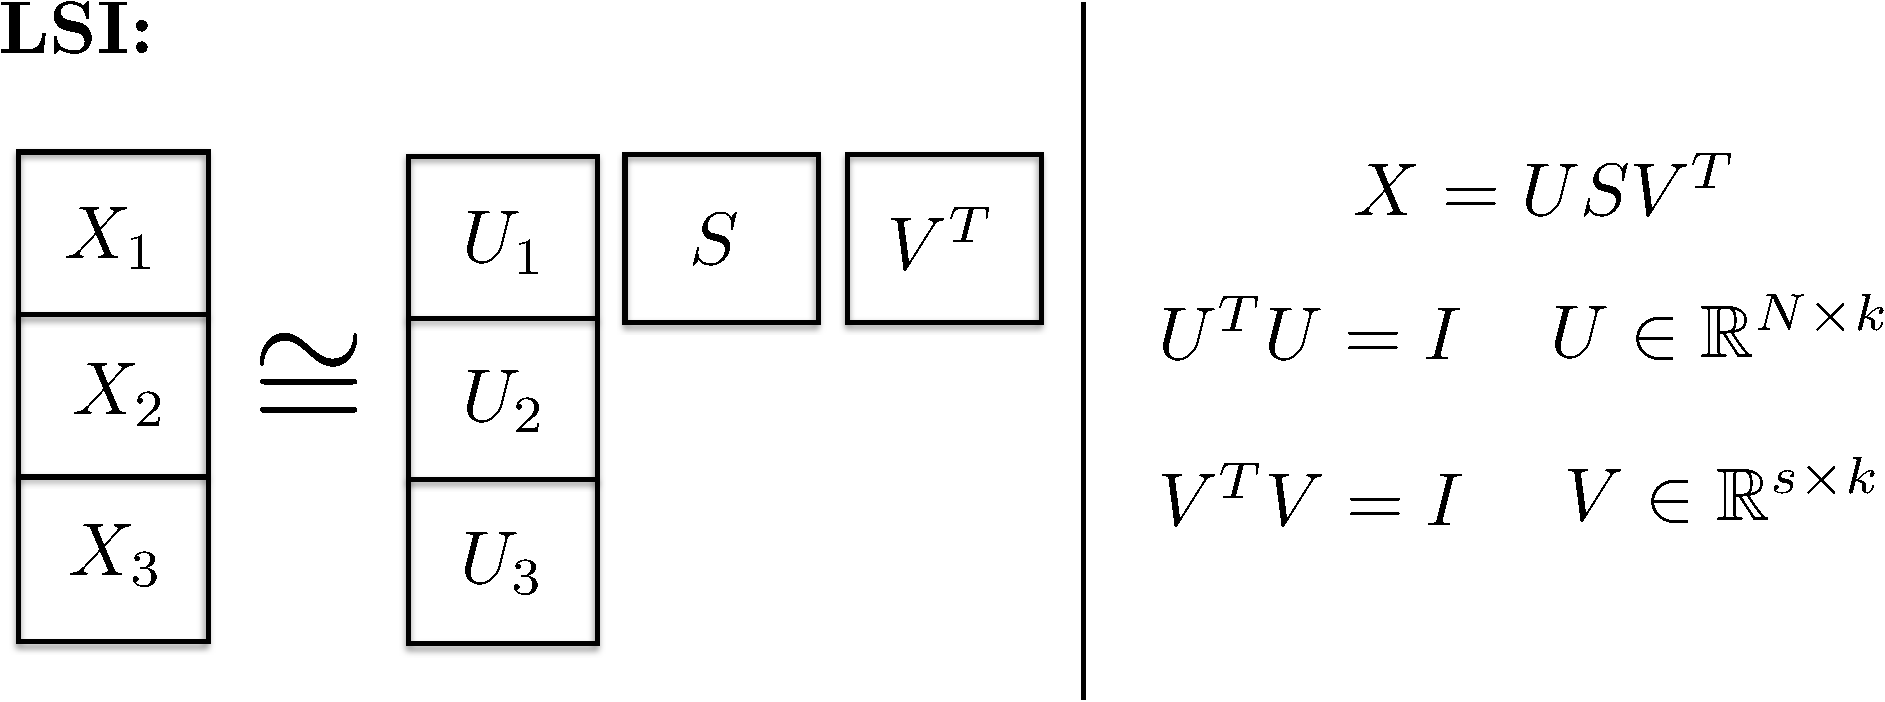
\includegraphics[width=10cm]{figures/lsi.pdf}
\caption{\label{fig:lsi} LSI multilingual corpus matrix decomposition.}
\end{figure}

The cross-lingual similarity functions are based on a rank-$k$ truncated SVD: $X \approx U \Sigma V^T,$ where $U \in \RR^{N \times k}$ are basis vectors of interest and $\Sigma \in \RR^{k \times k}$ is a truncated diagonal matrix of singular eigenvalues. An aligned basis is obtained by first splitting $U$ vertically according to the number of dimensions of each language: $U = [U_1^T \cdots U_m^T]^T$. Then, the same as with $k$-means clustering, we compute the pseudoinverses $P_i = (U_i^T U_i)^{-1} U_i^T$. The matrices $P_i$ are used to change the basis from the standard basis in $\RR^{n_i}$ to the basis spanned by the columns of $U_i$.

\paragraph{Implementation note}

  Since the matrix $X$ can be large we could use an iterative method like the Lanczos algorithm with reorthogonalization~\cite{golub} to find the left singular vectors (columns of $U$) corresponding to the largest singular values. It turns out that the Lanczos method converges slowly as the gap between the leading singular values is small. Moreover, the Lanczos method is hard to parallelize. Instead, we use a randomized version of the SVD~\cite{tropp} that can be viewed as a block Lanczos method. That enables us to use parallelization and speeds up the computation considerably.

To compute the matrices $P_i$ we used the QR algorithm~\cite{golub} to factorize $U_i$ as $U_i = Q_i R_i$, where $Q_i^TQ_i = I$ and $R_i$ is a triangular matrix. $P_i$ is then obtained by solving $R_i P_i = Q_i$.


\section{Hub language based CCA Extension}\label{sec:hublang}
Building cross-lingual similarity models based on comparable corpora is challenging for two main reasons. The first problem is related to missing alignment data: when a number of languages is large, the dataset of documents that cover all languages is small (or may even be empty). Even if only two languages are considered, the set of aligned documents can be small (an extreme example is given by the Piedmontese and Hindi Wikipedias where no inter-language links are available), in which case none of the methods presented so far are applicable.
 The second challenge is scale - the data is high-dimensional (many languages with hundreds of thousands of features per language) and the number of multilingual documents may be large (over one million in case of Wikipedia). The optimization problem posed by CCA is not
 trivial to solve: the covariance matrices themselves are prohibitively large to fit in memory (even storing a 100,000 by 100,000 element matrix requires 80GB of memory) and iterative matrix-multiplication based approaches to  solving generalized eigenvalue problems are required (the covariance matrices can be expressed as products of sparse matrices, which means we have fast matrix-vector multiplication).

We now describe an extension of CCA to more than two languages, which can be trained on large comparable corpora and can handle missing data.
 The extension we consider is based on a generalization of CCA to more than two views, introduced in~\cite{Kettenring}, namely the Sum of Squared Correlations SSCOR, which we will state formally later in this section. Our approach exploits a certain characteristic of the data, namely the \emph{hub language} characteristic (see below) in two
 ways: to reduce the dimensionality of the data and to simplify the optimization problem.

\paragraph{Hub language characteristic.}
In the case of Wikipedia, we observed that even though the training resources are scarce for certain language pairs, there often exists indirect training data. By considering a third language, which has training data with both languages in the pair,  we can use the composition of learned maps as a proxy. We refer to this third language as a hub language.

A \emph{hub language} is a language with a high proportion of non-empty documents in $D = \left\{d_1,..., d_{\ell}\right\}$. As we have mentioned, we only focus on multilingual documents that include at least two languages. The prototypical example in the case of Wikipedia is English. Our notion of the hub language could be interpreted in the following way.
If a non-English Wikipedia page contains one or more links to variants of the page in other languages, English is very likely to be one of them. That makes English a hub language.

We use the following notation to define subsets of the multilingual comparable corpus: let $a(i,j)$ denote the index set of all multilingual documents with non-missing data for the $i$-th and $j$-th language:  $$a(i,j) = \left\{k~ |~ d_k = (u_1,...,u_m), u_i \neq \emptyset, u_j \neq \emptyset \right\},$$ and let $a(i)$ denote the index set of all multilingual documents with non missing data for the $i$-th language.

We now describe a two step approach to building a cross-lingual similarity matrix. The first part is related to LSI and reduces the dimensionality of the data. The second step refines the linear mappings and optimizes the linear dependence between data.

\paragraph{Step 1: Hub language based dimensionality reduction.}

The first step in our method is to project $X_1, \ldots, X_m$ to lower-dimensional spaces without destroying the cross-lingual structure. Treating the nonzero columns of $X_i$ as observation vectors sampled from an underlying distribution $\mathcal{X}_i \in V_i = \RR^{n_i}$, we can analyze the empirical cross-covariance matrices:
$$C_{i,j} = \frac{1}{|a(i,j)|-1 }\sum_{\ell \in a(i,j)} (X_i^{\ell} - c_i)\cdot (X_j^{\ell} - c_j)^T,$$
 where $c_i = \frac{1}{a_i} \sum_{\ell \in a(i)}X_i^{\ell}$. By finding low-rank approximations of $C_{i,j}$ we can identify the subspaces of $V_i$ and $V_j$ that are relevant for extracting linear patterns between $\mathcal{X}_i$ and $\mathcal{X}_j$. Let $X_1$ represent the hub language corpus matrix. The LSI approach to finding the subspaces is to perform the singular value decomposition on the full $N \times N$ covariance matrix composed of blocks $C_{i,j}$. If $|a(i,j)|$ is small for many language pairs (as it is in the case of Wikipedia), then many empirical estimates $C_{i,j}$ are unreliable, which can result in overfitting. For this reason, we perform the truncated singular value decomposition on the matrix $C = [C_{1,2}  \cdots  C_{1,m}] \approx U S V^T$, where $U \in \RR^{n_1 \times k}, S \in \RR^{k \times k}, V \in \RR^{(\sum_{i=2}^m n_i) \times k}$. We split the matrix $V$ vertically in blocks with $n_2, \ldots, n_m$ rows: $V = [V_2^T  \cdots  V_m^T]^T$. Note that columns of $U$ are orthogonal but columns in each $V_i$ are not (columns of V are orthogonal). Let $V_1 := U$. We proceed by reducing the dimensionality of each $X_i$ by setting: $Y_i = V_i^T \cdot X_i$, where $Y_i \in \RR^{k\times N}$. To summarize, the first step reduces the dimensionality of the data and is based on CL-LSI, but optimizes only the hub language related cross-covariance blocks.

\paragraph{Step 2: Simplifying and solving SSCOR.}
The second step involves solving a generalized version of canonical correlation analysis on the matrices $Y_i$ in order to find the mappings $P_i$. The approach is based on the sum of squares of correlations formulation by Kettenring~\cite{Kettenring}, where we consider only correlations between pairs $(Y_1, Y_i), i >1$ due to the hub language problem characteristic.
We will present the original unconstrained optimization problem, then a constrained formulation based on the hub language problem characteristic. Then we will simplify the constraints and reformulate the problem as an eigenvalue problem by using Lagrange multipliers.

The original sum of squared correlations is formulated as an unconstrained problem:
\begin{equation*}
  \begin{aligned}
    & \underset{w_i \in \RR^{k}}{\text{maximize}}
    & & \sum_{i < j}^m  \rho(w_i^T Y_i, w_j^T Y_j)^2.
\end{aligned}
\end{equation*}
We solve a similar problem by restricting $i=1$ and omitting the optimization over non-hub language pairs.
Let $D_{i,i} \in \RR^{k \times k}$ denote the empirical covariance of $\mathcal{Y}_i$ and $D_{i,j}$ denote the empirical cross-covariance computed based on $\mathcal{Y}_i$ and $\mathcal{Y}_j$. We solve the following constrained (unit variance constraints) optimization problem:
\begin{equation}\label{squaredCorHubOriginal}
  \begin{aligned}
    & \underset{w_i \in \RR^{k}}{\text{maximize}}
    & & \sum_{i = 2}^m  \left(w_1^T D_{1,i} w_i \right)^2
    & \text{subject to}
    & & w_i^T D_{i,i} w_i = 1, \quad\forall i = 1,\ldots, m.
\end{aligned}
\end{equation}
The constraints $w_i^T D_{i,i} w_i$ can be simplified by using the Cholesky decomposition $D_{i,i} = K_i^T \cdot K_i$ and substitution: $y_i := K_i w_i$. By inverting the $K_i$ matrices and defining  $G_i := K_1^{-T} D_{1,i} K_i^{-1}$, the problem can be reformulated:
\begin{equation}\label{squaredCorHub}
  \begin{aligned}
    & \underset{y_i \in \RR^{k}}{\text{maximize}}
    & & \sum_{i = 2}^m  \left(y_1^T G_{i} y_i \right)^2
    & \text{subject to}
    & & y_i^T y_i = 1, \quad\forall i = 1,\ldots, m.
\end{aligned}
\end{equation}
A necessary condition for optimality is that the derivatives of the Lagrangian vanish. The Lagrangian of (\ref{squaredCorHub}) is expressed as:
$$  L(y_1, \ldots, y_m, \lambda_1, \ldots, \lambda_m) = \sum_{i = 2}^m  \left(y_1^T G_{i} y_i \right)^2 + \sum_{i=1}^m \lambda_i \left(y_i^T y_i - 1\right).$$
Stationarity conditions give us:
\begin{equation}\label{dLdx1}
 \frac{\partial}{\partial x_1} L = 0 \Rightarrow \sum_{i = 2}^m  \left(y_1^T G_{i} y_i \right) G_i y_i + \lambda_1 y_1 = 0,
\end{equation}
\begin{equation}\label{dLdxi}
\frac{\partial}{\partial x_i} L = 0 \Rightarrow \left(y_1^T G_{i} y_i \right) G_{i}^T y_1 + \lambda_i y_i = 0,~i > 1.
\end{equation}
Multiplying the equations (\ref{dLdxi}) with $y_i^T$ and applying the constraints, we can eliminate $\lambda_i$ which gives us:
\begin{equation}\label{eqy1yi}
G_{i}^T y_1 = \left(y_1^T G_{i} y_i \right) y_i,~i > 1.
\end{equation}
Plugging this into (\ref{dLdx1}), we obtain an eigenvalue problem:
$$\left( \sum_{i = 2}^m G_i G_{i}^T \right) y_1 + \lambda_1 y_1 = 0.$$
The eigenvectors of $\left( \sum_{i = 2}^m G_i G_{i}^T \right)$ solve the problem for the first language. The solutions for $y_i$ are obtained from (\ref{eqy1yi}): $y_i := \frac{G_{i}^T y_1}{\| G_{i}^T y_1 \|}$.
Note that the solution (\ref{squaredCorHubOriginal}) can be recovered by: $w_i := K_i^{-1} y_i$. The linear transformation of the $w$ variables are thus expressed as:
$$ Y_1 := \text{eigenvectors of} \sum_{i = 2}^m G_i G_{i}^T, $$
$$ W_1 = K_1^{-1} Y_1 $$
$$ W_i = K_i^{-1} G_{i}^T Y_1 N,$$
where $N$ is a diagonal matrix that normalizes $G_{i}^T Y_1$, with $N(j,j) := \frac{1}{\|G(_{i} Y_1(:,j)\|}$.

\paragraph{Remark.} The technique is related to  Generalization of Canonical Correlation Analysis (GCCA) by Carroll~\citeyear{Carroll}, where an unknown group configuration variable is defined and the objective is to maximize the sum of squared correlations between the group variable and the others. The problem can be reformulated as an eigenvalue problem. The difference lies in the fact that we set the unknown group configuration variable as the hub language, which simplifies the solution. The complexity of our method is $O(k^3)$, where $k$ is the reduced dimension from the LSI preprocessing step, whereas solving the GCCA method scales as $O(s^3)$, where $s$ is the number of samples (see~\cite{gifi}). Another issue with GCCA is that it cannot be directly applied to the case of missing documents.

To summarize, we first reduced the dimensionality of our data to $k$-dimensional features and then found a new representation (via linear transformation) that maximizes directions of linear dependence between the languages. The final projections that enable mappings to a common space are defined as: $P_i(x) = W_i^T V_i^T x.$

